\section{Evaluation}
\label{sec:evaluation}

% \begin{figure*}
%     \centering
%     \begin{minipage}[b]{0.49\textwidth}
%         \centering
%         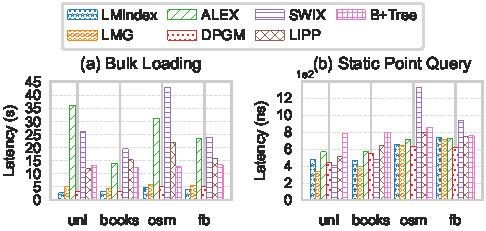
\includegraphics[width=1\textwidth]{vldbj_figs/bulk_purepq.pdf}
%         \caption{Bulk loading latency and static query latency.}
%         \label{fig:bulk_pquery}
%     \end{minipage}
%     \begin{minipage}[b]{0.49\textwidth}
%         \centering
%         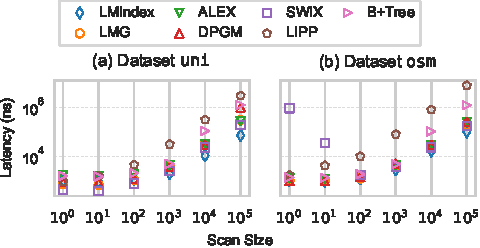
\includegraphics[width=1\textwidth]{vldbj_figs/pure_range_query.pdf}
%         \caption{Static range query latency under varying scan ranges.}
%         \label{fig:pure_rq}
%     \end{minipage}
% \end{figure*}

\subsection{Experimental Setup}
All code is implemented in C++ (available at \url{github.com/Nuiqv/LMIndex}). Our single-threaded experiments are conducted on an Ubuntu 24.04 machine with an AMD R9 7945HX 2.5GHz CPU and 64GB RAM, compiled with gcc -O3 -march=native.

\subsubsection{Baseline} We evaluate LMIndex and LMG against five representative baselines. Shared parameters such as the error threshold are aligned for fairness and others remain default to simulate real-world scenarios that are difficult to tune. (1) Dynamic PGM Index (DPGM) \cite{pgm20} is the update-capable variant of PGM, using the same error threshold~$\varepsilon$ as LMIndex. (2) ALEX~\cite{alex20} adopts gapped arrays with model-based insertion and exponential search. We set its max node size equal to our max layer size $\mathit{L}$. (3) SWIX~\cite{swix24} is optimized for streaming data with a flat routing layer and strong random access support. We use default settings. (4) STX B+Tree~\cite{stxbtree19} serves as the traditional baseline, evaluated with its default configuration. (5) LIPP \cite{lipp21, learned23} adopts a Zero Error strategy, which eliminates the need for error correction search steps during the query process. LMIndex is configured with a max layer size $\mathit{L}=2^{16}$, initial error threshold $\varepsilon=64$. LMG inherits the parameters of LM without employing an additional buffer; instead, it utilizes a gapped array with an expansion rate of $\tau=0.5$ to accommodate updates. This configuration is a balanced trade-off, and parameter sensitivity is discussed in Section~\ref{sec:param-eval}.

\subsubsection{Datasets}
All experiments are conducted on four representative datasets: a synthetic dataset with uniform distribution and three real-world datasets from the SOSD benchmark~\cite{sosd20}. The Uniform dataset (\texttt{uni}, 200M keys) contains keys drawn from a globally and locally linear distribution. The Amazon Books dataset (\texttt{books}, 200M keys) exhibits global non-linearity with partially linear local distributions. The Open Street Map dataset (\texttt{osm}, 200M keys) is both globally and locally non-linear. The Facebook user IDs dataset (\texttt{fb}, 200M keys) is mostly linear but includes a small number of large outliers. All keys are of the $64$-bit unsigned integer type and contain no duplicate values, consistent with prior studies or the open-source codebases of learned baselines.

% debug now
\subsubsection{Workloads}
We evaluate our approach primarily based on the following three categories of workloads. First, we consider static (read-only) workloads. For these scenarios, we perform read-only operations both immediately after bulk loading the entire dataset and after a specific volume of insertions. Second, we examine mixed read-write workloads, with the insertion frequencies set to 20\%, 40\%, 60\%, and 80\%, respectively. In these experiments, we initially bulk load 50\% of the data and subsequently execute 100M random read-write operations. Third, we evaluate range queries with lengths varying from $10^0$ to $10^5$. For these queries, we select 10K random starting keys and report the average latency. We evaluate LM exclusively under static scenarios. In addition, for point queries, we select 10M random keys and measure the latency.

\subsubsection{Metrics}
We measure time using average operation latency, recorded at nanosecond resolution with C++ \texttt{std::chrono}. Hardware-backed timers minimize instrumentation overhead to less than 5\%, rendering the interference with experimental results virtually negligible \cite{paoloni2010, najafi2021systems}. For memory, we track historical physical peak usage \texttt{VmHWM}. Unlike theoretical size, VmHWM represents the minimum spatial resources required for operation throughout the entire lifecycle. To ensure accuracy, all memory measurements subtract the initial usage before bulk loading.

\subsection{Evaluation of Diverse Dimensions}
We evaluated six key performance dimensions: bulk loading, point queries, range queries, stability, space usage, and updates. These dimensions characterize the fundamental lifecycle of an index, and critically impact its overall time-space efficiency.

\begin{figure*}
    \centering
    \begin{minipage}[b]{0.51\textwidth}
        \centering
        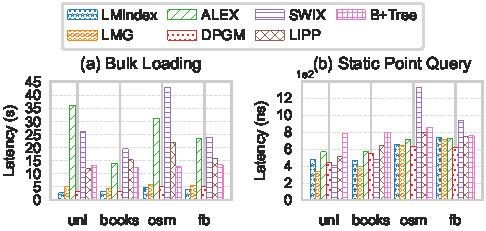
\includegraphics[width=1\textwidth]{vldbj_figs/bulk_purepq.pdf}
        \caption{Bulk loading latency and static query latency.}
        \label{fig:bulk_pquery}
    \end{minipage}
    \begin{minipage}[b]{0.47\textwidth}
        \centering
        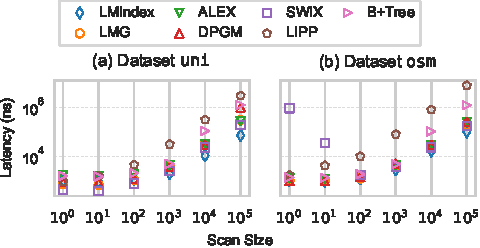
\includegraphics[width=1\textwidth]{vldbj_figs/pure_range_query.pdf}
        \caption{Static range query latency under varying scan ranges.}
        \label{fig:pure_rq}
    \end{minipage}
    \begin{minipage}[b]{1\textwidth}
        \centering
        \begin{subfigure}[b]{0.9\textwidth}
        \centering
        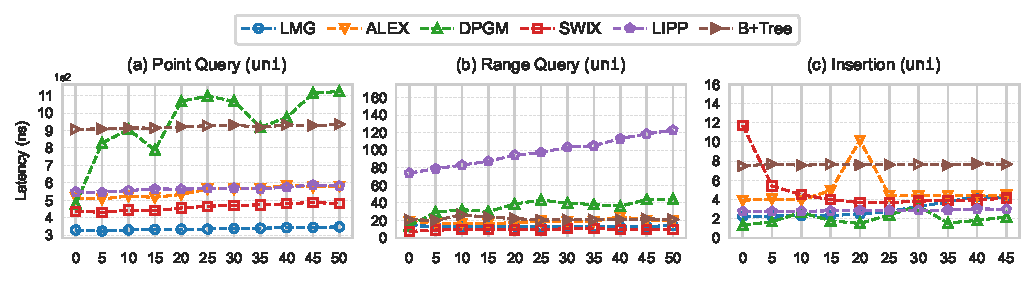
\includegraphics[width=1\textwidth]{vldbj_figs/stability_test_avg.pdf}
        \end{subfigure}
        \begin{subfigure}[b]{0.9\textwidth}
            \centering
            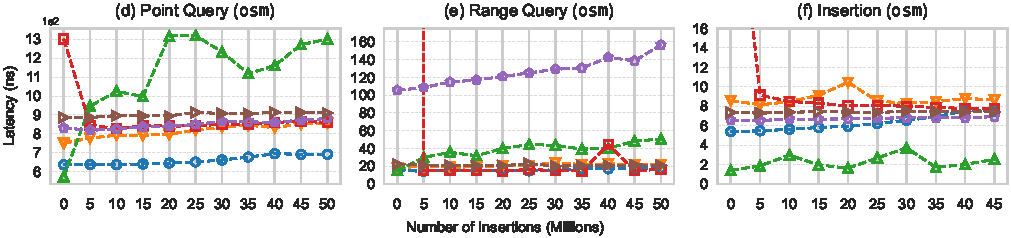
\includegraphics[width=1\textwidth]{vldbj_figs/stability_test_osm.pdf}
        \end{subfigure}
        \caption{Index stability and dynamic performance during continuous insertions (0-50M).}
        \label{fig:stability}
    \end{minipage}
\end{figure*}

% \begin{figure*}
%     \centering
%     \begin{subfigure}[b]{0.9\textwidth}
%     \centering
%     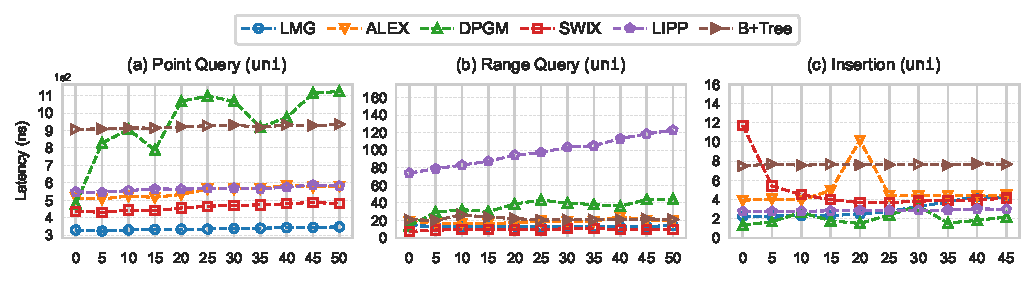
\includegraphics[width=1\textwidth]{vldbj_figs/stability_test_avg.pdf}
%     \end{subfigure}
%     \begin{subfigure}[b]{0.9\textwidth}
%         \centering
%         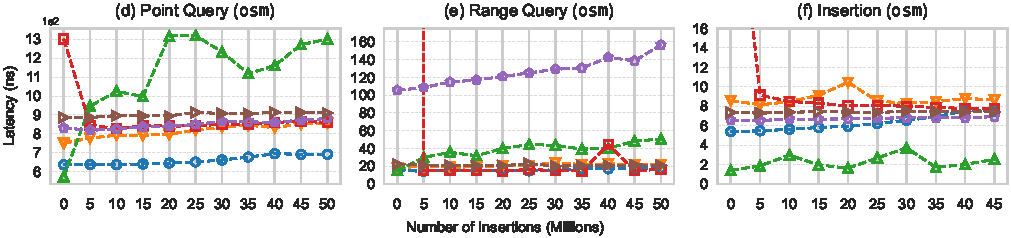
\includegraphics[width=1\textwidth]{vldbj_figs/stability_test_osm.pdf}
%     \end{subfigure}
%     \caption{Index stability and dynamic performance during continuous insertions (0-50M).}
%     \label{fig:stability}
% \end{figure*}

\subsubsection{Bulk Loading}
Bulk loading serves as a practical mechanism to initialize deployments and restore index quality after severe data distribution shifts. Figure \ref{fig:bulk_pquery}a reports the execution time across datasets, where our foundational structure, LMIndex, demonstrates superior initialization efficiency. Specifically, LMIndex achieves average speedups of 7.37$\times$ and 7.55$\times$ over top-down models like ALEX and SWIX, 4.37$\times$ over LIPP, 3.59$\times$ over B+Trees, and 1.14$\times$ over DPGM. Due to the gapped array allocation strategy, LMG slightly increases latency, being approximately 1.45$\times$ slower. Notably, the efficiency of both LMIndex and LMG does not exhibit drastic fluctuations across different data distributions.

The shared efficiency of LM and LMG inherently stems from the Bottom-Up training strategy. By greedily constructing segments through a single-pass scan over the sorted data ($O(N)$ complexity), our framework bypasses the expensive global data profiling required by other designs. Conversely, the structural bottlenecks of competing strategies become evident during initialization. Top-Down models (e.g., ALEX, SWIX) mandate recursive, multi-pass dataset scans to partition data and fit global models, resulting in significant loading delays. Similarly, Zero Error architectures like LIPP require the calculation and pre-allocation of a substantial number of contiguous empty slots, which diminishes bulk loading efficiency.

\subsubsection{Point Query}
\label{sec:point_query}
Point query execution time represents a fundamental metric for evaluating the retrieval efficiency of an index structure. Figure \ref{fig:bulk_pquery}b reports the static latency across read-only datasets. LMG demonstrates highly competitive retrieval performance, achieving average speedups of 1.30$\times$ over ALEX, 1.34$\times$ over LIPP, and 1.67$\times$ over B+Trees, while operating 1.15$\times$ faster than the base LMIndex. This baseline efficiency is primarily attributed to the Leaf-only Error strategy. By leveraging OETA to compress segment error thresholds, LMG further reduces error correction overhead, which is particularly effective on datasets with substantial latent compression potential (e.g., \texttt{uni}, \texttt{books}).

The performance differentiation becomes more pronounced under dynamic workloads with continuous insertions. As illustrated in the stability analysis (Figure \ref{fig:stability}a, \ref{fig:stability}d), competing architectures experience various degrees of performance degradation after 50M continuous insertions. For instance, DPGM, which exhibits static latency comparable to LMG, becomes 1.68$\times$ and 2.80$\times$ slower than LMG on the \texttt{osm} and \texttt{uni} datasets, respectively. In contrast, LMG sustains its point query efficiency throughout the dynamic lifecycle, extending its speedup over models like ALEX and LIPP to 1.63$\times$/1.23$\times$ and 1.68$\times$/1.28$\times$ on the \texttt{uni}/\texttt{osm}. The robustness and efficiency of point queries demonstrate that LM effectively maintains high indexing quality during updates.

\subsubsection{Range Query}
\label{sec:range_query}
In modern database systems, range queries serve as the foundational primitives for executing complex analytical operations, including relational joins and multi-dimensional aggregations (e.g., GROUP BY). Figure \ref{fig:pure_rq} reports the static range query latency across varying scan ranges (from $10^0$ to $10^5$). As anticipated, LMIndex exhibits the highest average range queries efficiency due to its strictly dense memory layout, executing slightly faster than LMG (1.13$\times$ faster). The gapped array allocation in LMG introduces a predictable, marginal overhead during sequential scans; nevertheless, LMG sustains a significant advantage over other architectures, achieving average speedups of 1.39$\times$ over ALEX, 1.30$\times$ over DPGM, and 2.54$\times$ over B+Trees. Crucially, zero error structures like LIPP incur a severe 11.41$\times$ slowdown compared to LMG. This execution penalty stems from the massive, dispersed empty slots required to enforce strict physical-to-prediction alignments, which heavily disrupt spatial locality and induce frequent cache misses during sequential traversals.

Regarding dynamic range queries, we evaluates the performance of $100$ range queries following continuous updates. As shown in Figure \ref{fig:stability}b, Figure \ref{fig:stability}e, indexes relying on fragmented experience notable performance degradation. Specifically, LIPP suffers a 7.65$\times$ slowdown on average due to progressive memory fragmentation. Similarly, DPGM (2.52$\times$ slowdown on average) experiences scan degradation because its LSM-tree style updates require traversing and merging data across multiple levels. Conversely, by leveraging efficient traversal of sequentially linked leaf nodes, B+Tree and ALEX are, on average, $1.48\times$ and $1.37\times$ slower, respectively. SWIX further strengthens its advantage through a completely flat segment indexing structure, outperforming LMG by $1.39\times$ on the \texttt{uni} dataset; however, it exhibits instability on the complex \texttt{osm} dataset, performing $1.86\times$ slower than LMG. LMG shares these structural advantages. The LM structure exhibits the characteristics of a flat array, while the segment list is ordered and linked similarly to a B+Tree. Consequently, LMG avoids severe fragmentation and the overhead of cross-level merging, ensuring both robustness and efficiency for range queries.

\begin{figure*}
    \centering
    \begin{minipage}[b]{0.32\textwidth}
        \centering
        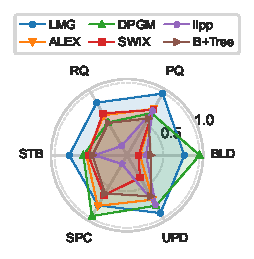
\includegraphics[width=1\textwidth]{vldbj_figs/radar.pdf}
        \caption{Comprehensive evaluation of multi-dimensional performance.}
        \label{fig:radar}
    \end{minipage}
    \begin{minipage}[b]{0.65\textwidth}
        \centering
        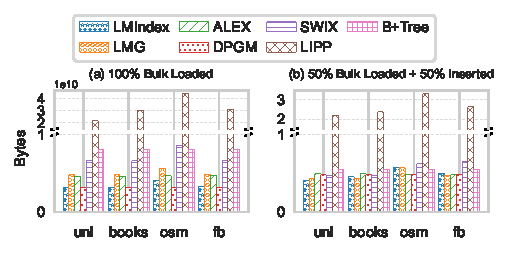
\includegraphics[width=1\textwidth]{vldbj_figs/space_test.pdf}
        \caption{Space footprint comparison under static initialization versus dynamic workload conditions.}
        \label{fig:space}
    \end{minipage}
    \begin{minipage}[b]{1\textwidth}
        \centering
        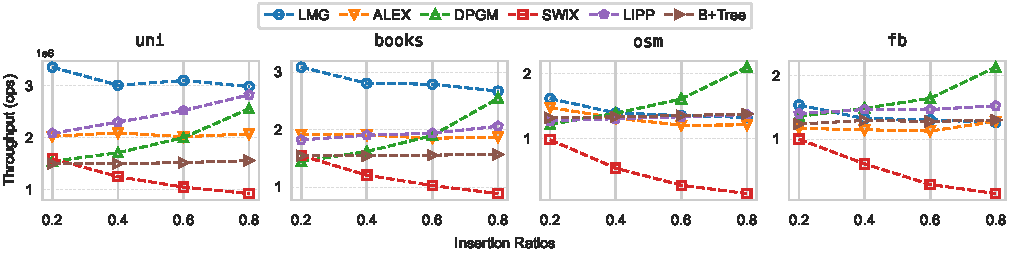
\includegraphics[width=1\textwidth]{vldbj_figs/update_test.pdf}
        \caption{Overall throughput under mixed read-write workloads with varying insertion ratios (0.2 to 0.8).}
        \label{fig:update}
    \end{minipage}
\end{figure*}

\subsubsection{Stability}
\label{sec:stability}
Maintaining performance stability during continuous updates is a fundamental capability for the long-term deployment of index structures. Figure \ref{fig:stability} trace the latency evolution of point queries, range queries, and insertions across a continuous insertion workload. As analyzed in Sections \ref{sec:point_query} and \ref{sec:range_query}, LMG demonstrates sustained read efficiency throughout the operational lifecycle. From a stability perspective, this confirms the structural robustness of the LM in dynamic scenarios, which additionally benefits from the inherent robustness of the underlying hybrid search.

Focusing on the insertion operations (Figure \ref{fig:stability}c, \ref{fig:stability}f), DPGM exhibits the lowest execution latency, operating at a 1.87$\times$ faster compared to LMG. This insertion efficiency directly derives from its LSM-Tree style update strategy, which sequentially buffers incoming records without querying for positioning. However, as established in previous sections, this mechanism inherently penalizes query performance. Conversely, traditional B+Trees maintain a highly stable insertion curve due to their standardized node-splitting mechanism, yet their absolute execution time remains consistently high, averaging a 1.94$\times$ slowdown relative to LMG. Other learned baselines, including ALEX, SWIX, and LIPP, record average execution slowdowns of 1.58$\times$, 1.84$\times$, and 1.04$\times$, respectively, placing LMG's overall insertion performance in a highly competitive position.

Furthermore, it can be observed that the insertion latency of LMG gradually increases during the later stages. This trend represents an expected structural phenomenon. Initially, the gapped array allocation efficiently absorbs incoming records. As the total data volume grows and the pre-allocated gaps reach capacity, the framework increasingly triggers local segment retrains. Consequently, the frequency of these retrains naturally scales with the data volume before eventually converging to a stable rate. Nevertheless, by strictly confining these necessary retrains to localized segments, LMG successfully balances insertion costs with robust long-term read efficiency.

\subsubsection{Space Usage}
Figure \ref{fig:space} reports the historical physical peak memory usage (\texttt{VmHWM}) under static and dynamic initialization scenarios. In the 100\% bulk loaded setting (Figure \ref{fig:space}a), the spatial footprint of LMG is 1.47x that of LMIndex on average. This value is very close to the theoretical expansion of the gapped array in LMG (i.e., $(1 + \tau = 1.5)\times$). This confirms the inherent space efficiency of the base LM architecture and indicates that LMG's spatial footprint is primarily dominated by its underlying gapped array. Among other baselines, DPGM exhibits the most compact static footprint (0.63$\times$) owing to its RMI-style structure (Only the model parameters need to be stored) and dense segment layout. ALEX operates at 0.93$\times$, while SWIX and B+Trees consume 1.40$\times$ and 1.60$\times$, respectively. As established in previous sections, LIPP incurs a massive 6.26$\times$ overhead due to the physical sparsity mandated by its zero error strategy.

The spatial dynamics shift notably under continuous insertions (Figure \ref{fig:space}b). Both DPGM and LMIndex see their relative space consumption increase to 1.02$\times$ compared to LMG, highlighting their spatial instability and the fragmentation costs incurred during continuous structural modifications. Crucially, while top-down architectures like ALEX can also employ gapped arrays to absorb updates, LMG ultimately consumes less space than ALEX (1.03$\times$), SWIX (1.17$\times$), and B+Trees (1.17$\times$). This advantage stems from the inherent space efficiency of the foundational LM structure, which naturally naturally fits the underlying segment distribution and does not require a lot of routing metadata. LIPP remains highly inefficient at 5.48$\times$. Consequently, LMG's structural design effectively prevents severe memory inflation throughout its lifecycle.

\subsubsection{Update Performance}
Distinct from the stability evaluated in Section \ref{sec:stability}, this section assesses index throughput under mixed workloads, with write ratios varying from 0.2 to 0.8. Averaged across all datasets and workload configurations, LMG demonstrates highly competitive overall throughput, operating 1.31$\times$ faster than ALEX, 1.49$\times$ over B+Trees, 1.19$\times$ over LIPP, 1.26$\times$ over PGM, and 3.50$\times$ over SWIX. Specifically, LMG consistently achieves the highest throughput on the \texttt{uni} and \texttt{books} datasets, validating its efficiency under these distributions.

On the \texttt{osm} and \texttt{fb} datasets, LMG slightly trails DPGM and LIPP under specific mixed workloads. This performance variance is primarily driven by the distinct structural characteristics of the baselines. For example, the LSM-tree-style buffer in DPGM enables direct insertions without requiring query routing; however, distributing data across multiple levels degrades the efficiency of subsequent reads. Furthermore, LMG exhibits a slight throughput reduction under specific heavy-read workloads. This behavior stems from our conservative segment retraining strategy. To strictly guarantee read efficiency and preserve local error bounds, LMG proactively triggers segment retrains before the pre-allocated gaps are fully exhausted. While this deliberate architectural trade-off introduces a predictable structural overhead as write operations occur, it successfully ensures bounded, long-term operational stability without compromising read performance.

\subsubsection{Holistic Performance and Multi-dimensional Balance}
Figure \ref{fig:radar} synthesizes the holistic performance of the evaluated indexes through a normalized radar chart (score from 0.0 to 1.0). For most dimensions (e.g., Bulk Loading and Space Usage), normalized scores are derived by averaging relative performance metrics across all datasets. To accurately capture long-term index stability, the Stability (STB) dimension is quantified using the Area Under the Curve (AUC), defined as $AUC = \int_{0}^{50M} Latency(x) \,dx$. This formulation effectively penalizes unpredictable latency spikes and sustained execution delays over the continuous insertion lifecycle. Furthermore, the Point Query (PQ) and Range Query (RQ) dimensions aggregate both static and dynamic workloads from STB to reflect a comprehensive operational lifecycle.

The resulting visualization exposes the severe multi-dimensional trade-offs inherent in existing baselines. For instance, while DPGM achieves near-optimal normalized scores in Bulk Loading (1.000) and Space Consumption (0.969), its structural rigidity severely penalizes its Range Query (0.520) and Stability (0.602) performance. Similarly, zero error architectures like LIPP catastrophically compromise Space (0.141) and Range Queries (0.148) to maintain read limits. In contrast, LMG yields the most expansive and balanced performance polygon. By consistently sustaining high normalized scores across all six dimensions (ranging from 0.789 to 0.981), LMG empirically validates its core design philosophy: avoiding catastrophic degradation in any single metric to deliver robust, general-purpose efficiency across diverse and dynamic database workloads.

\begin{figure*}
    \centering
    \begin{minipage}[b]{0.5\textwidth}
        \centering
        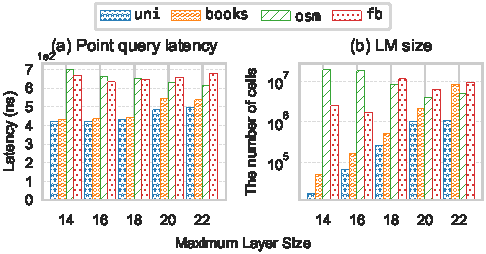
\includegraphics[width=\linewidth]{vldbj_figs/max_layer_size.pdf}
        \caption{Evaluation of point query performance and LM size under different maximum layer sizes ($2^{14}$ to $2^{22}$) for LM.}
        \label{fig:max_layer_size}
    \end{minipage}
    \begin{minipage}[b]{0.48\textwidth}
        \centering
        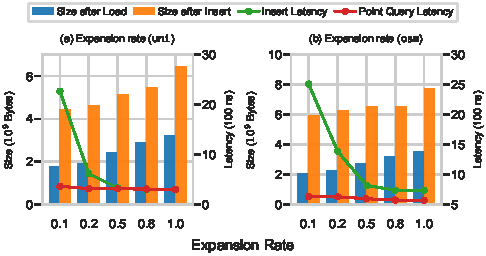
\includegraphics[width=1\textwidth]{vldbj_figs/expansion_rate.pdf}
        \caption{Impact of expansion rate on LMG in terms of point query, insert and space.}
        \label{fig:expansion_rate}
    \end{minipage}
    % \hfill
    \begin{minipage}[b]{0.27\textwidth}
        \centering
        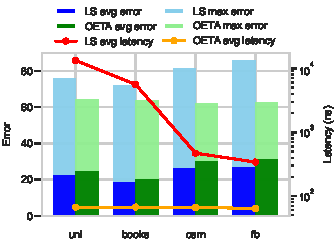
\includegraphics[width=\linewidth]{vldbj_figs/oeta_vs_ls.pdf}
        \caption{Analysis of OETA and Least Squares.}
        \label{fig:oeta_vs_ls}
    \end{minipage}
    \begin{minipage}[b]{0.27\textwidth}
        \centering
        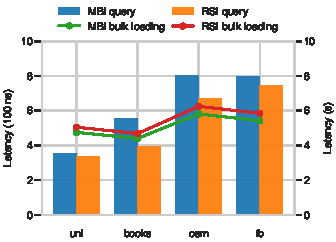
\includegraphics[width=\linewidth]{vldbj_figs/lmg_insert_comparison.pdf}
        \caption{Comparison of gap allocation strategies.}
        \label{fig:lmg_insert_comparison}
    \end{minipage}
    % \hfill
    \begin{minipage}[b]{0.45\textwidth}
        \centering
        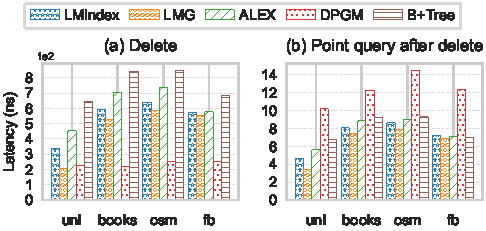
\includegraphics[width=0.86\linewidth]{vldbj_figs/delete_test.pdf}
        \caption{Deletion efficiency and its impact on query performance.}
        \label{fig:delete_test}
    \end{minipage}
\end{figure*}

\subsection{Detailed Evaluation}
\subsubsection{Parameter Evaluation}
\label{sec:param-eval}
We evaluate the impact of the maximum layer size $\mathit{L}$ on LMIndex, as well as the expansion rate $\tau$ on LMG.

\textbf{Max Layer Size.} Figure \ref{fig:max_layer_size} evaluates the sensitivity of the LM structure to its maximum layer size $\mathit{L}$ (from $2^{14}$ to $2^{22}$). Crucially, point query latency exhibits relative consistency across all $\mathit{L}$ values, demonstrating that retrieval efficiency is structurally robust and insensitive to parameter tuning. Regarding space usage, the size of LM remains relatively stable for complex data distributions (e.g., \texttt{books}, \texttt{osm}, and \texttt{fb}). Conversely, on the relatively linear and uniform dataset \texttt{uni}, expanding $\mathit{L}$ increases the number of cells per segment, leading to a significant increase in index size. However, despite this trend, the absolute LM size on the \texttt{uni} dataset remains the lowest among all evaluated distributions, and it stabilizes within the $2^{20}$ to $2^{22}$ parameter range. Overall, adjusting $\mathit{L}$ across a vast parameter space achieves relatively stable performance; a smaller $\mathit{L}$ can yield a slight advantage on more linear distributions, though the absolute magnitude of this improvement is marginal (compare to complex distributions). This further verifies the structural robustness of LM.

\textbf{Expansion Rate.} The expansion rate $\tau$ determines the proportion of reserved gaps in the data array, influencing both memory footprint and update/query performance. As shown in Figure \ref{fig:expansion_rate}, increasing $\tau$ initially reduces insertion latency, but the benefits saturates once most updates are absorbed by existing gaps. Query latency also improves slightly due to fewer correction steps, though the gain quickly saturates, especially on datasets with linear distributions like \texttt{uni}. Meanwhile, memory usage rises steadily with larger $\tau$, reflecting the overhead of excess reserved gaps. Therefore, selecting $\tau$ requires balancing update performance against memory overhead. Overall, the magnitude of $\tau$ is linearly correlated with space consumption. Regarding queries, the impact of $\tau$ remains relatively stable; for insertions, a smaller $\tau$ is preferable. However, we identify $0.5$ as a ``sweet spot'': across two datasets with vastly different distributions, it serves as the inflection point where the slope of insertion latency begins to flatten, while still maintaining a moderate spatial footprint.

\subsubsection{Gap Allocation Strategy}
We compare two gap allocation strategies within LMG: model-based insertion \cite{alex20} and reserved-space insertion. As shown in Figure \ref{fig:lmg_insert_comparison}, the reserved-space insertion incurs slightly higher bulk load time due to more complex gap placement. However, it consistently delivers better query performance by pre-allocating gaps more evenly across array. This reduces average correction length and improves search performance. Overall, given the efficient bulk loading process of LMG, the small increase in load time is an acceptable trade-off for stronger runtime performance.

\subsubsection{OETA vs. Least Squares} 
\label{sec:oeta_vs_ls}
% We compare OETA with the classic least squares (LS) method across three metrics: average maximum error per segment, average mean error per segment, and algorithm runtime. As shown in Figure \ref{fig:oeta_vs_ls}, OETA outperforms LS by reducing the average maximum error by 15.4\%–26.6\% while incurring only 0.5\%–18\% of LS’s runtime. These improvements align with OETA's theoretical design, which directly minimizes the maximum segment error to accelerate binary search. Moreover, this efficiency makes OETA suitable for time-sensitive scenarios, offering an alternative approach to computing model parameters for other learned indexes.

We evaluate the training efficacy of OETA against the standard least squares (LS) baseline by measuring three key metrics: average maximum error per segment, average mean error per segment, and algorithm runtime. As shown in Figure \ref{fig:oeta_vs_ls}, OETA consistently yields tighter error bounds. Compared to the LS baseline, OETA improves the average mean error by 12.5\% on average and reduces the average maximum error by 15.4\% to 26.6\%. This mean/maximum error trade-off is particularly effective when we employ maximum error sensitive binary search. In terms of runtime, OETA demonstrates fundamental advantages in computational efficiency and stability. Experimental results indicate that OETA consumes only 0.5\% to 18\% of the runtime required by LS. Crucially, while the performance of the Least Squares (LS) method exhibits high variance, OETA maintains a nearly consistent low overhead across diverse data distributions. The experimental results manifest the characteristics of an $O(1)$ algorithm, aligning with our theoretical derivations. Furthermore, this efficiency renders OETA more suitable for time-sensitive scenarios, providing an alternative approach for computing model parameters in other learned indexes.

\begin{table}
  \caption{Statistics of Linear Map}
  \small
  \begin{tabular}{lcccc}
  % \begin{tabular}{lllll}
    \toprule
     &\textbf{uni}&\textbf{books}&\textbf{osm}&\textbf{fb}\\
    \midrule
    \textbf{Avg update latency (ns)}	& 156.86 & 159.99 & 280.13 & 111.05\\
    \textbf{Avg layer size}			& 61504	&671.6	&3333	&20.4\\
    \textbf{Avg search depth}			& 0	&0.004	&0.989	&2.184\\
    \textbf{Avg segment's cells}			& 4.7	&5.6	&135.4	&3.6\\
    \textbf{Max layer depth}			& 0	&2	&2	&3\\
    \textbf{Num of layer} 			& 1	&249	&15704	&93025\\
    \textbf{LM building time / total}	    & 0.02\% & 0.16\% & 6.16\% & 3.08\%\\
    \textbf{LM space usage / total}	    & 0.066\% & 0.17\% & 15.7\% & 1.73\%\\
  \bottomrule
  \label{tab:lm_info}
\end{tabular}
\end{table}
\subsubsection{Linear Map Evaluation} 
\label{sec:lm_eval}
Table \ref{tab:lm_info} presents key statistics of LM, except update latency measured under a 50\% random insertion workload and all other metrics collected after fully loading each dataset. The root layer is defined as depth 0. Across datasets, LM exhibits consistently low and stable update latency. Most keys are located within 1 layer, with the \texttt{fb} dataset being an exception due to the segments containing a small number of large outliers placed at the root. Owing to the flat layer structure and the training-free model design, LM achieves almost negligible build time, accounting for just 0.02\%–6.16\% of total index construction time.


\subsubsection{Delete Evaluation}
Figure \ref{fig:delete_test} evaluates the deletion efficiency by removing 50\% of the dataset and measuring the subsequent point query latency. In terms of sheer deletion speed, DPGM exhibits the lowest latency. This efficiency derives directly from its LSM-tree-style mechanism, which rapidly appends tombstone markers without verifying the actual existence of the target keys. However, this blind insertion strategy inevitably penalizes subsequent read operations, causing DPGM to perform 2.05$\times$ slower than LMG in post-deletion queries on average. Conversely, LMG employs a more balanced approach that combines in-place tombstone marking with localized segment merging and retraining. While this structural maintenance introduces a slight latency overhead during the deletion phase (though LMG still operates 1.45$\times$ and 1.85$\times$ faster than ALEX and B+Trees, respectively), it effectively bounds the deterioration of prediction accuracy. Ultimately, LMG strikes a robust architectural trade-off, efficiently accommodating massive deletions while preserving long-term query stability.

\section{Discussion and Extensibility}
\label{sec:extend}
While the current LMG architecture is fundamentally designed as a foundational framework to achieve multi-dimensional performance balance for complex workloads, its highly decoupled hybrid structure remains inherently extensible. By isolating the routing logic from the underlying physical data layout, LMG provides a versatile blueprint capable of supporting a broader spectrum of complex database operations and query paradigms.

\textbf{Duplicate Keys Support.} LMG could naturally accommodate duplicate keys by pushing the handling logic down to the localized segments. In this configuration, the upper-level LM structure would solely manage segment distribution information, remaining entirely oblivious to key duplication. During the localized model training phase, the segment would train its model exclusively on unique keys and their physical positions, thereby ensuring prediction accuracy and bounding inference errors. Consequently, point queries could efficiently locate the target primary key within the local segment, and subsequent range scans could seamlessly traverse the associated value lists without disrupting the contiguous segment alignment.

\textbf{Concurrent Operations.} To support multi-threaded database workloads, LMG could integrate standard concurrency control protocols. Because structural modifications (SMOs), such as gap allocation and segment retraining, are strictly confined to local boundaries within our hybrid architecture, LMG would be well-suited to employ fine-grained, segment-level latching (e.g., read-write locks) for the bottom data layer. This localized absorption would drastically minimize lock contention during highly concurrent insertions. Simultaneously, the upper routing layer could be protected using Optimistic Concurrency Control (OCC) or versioned locks, ensuring that read transactions traverse the hierarchy without heavy synchronization overheads.

\textbf{Vector and High-Dimensional Queries.} Although originally optimized for 1D scalar keys, LMG could be adapted to support high-dimensional vector searches. This extension could be achieved by employing order-preserving mappings, such as Space-Filling Curves (e.g., Z-order or Hilbert curves) or Locality-Sensitive Hashing (LSH), to project multi-dimensional vectors into single-dimensional scalar keys. LMG could subsequently be constructed over these mapped keys. Under this paradigm, complex high-dimensional proximity evaluations or $k$-nearest neighbor ($k$-NN) candidate retrievals would effectively be transformed into localized 1D range scans, allowing the system to leverage LMG's robust sequential scanning efficiency.